% move all configuration stuff into includes file so we can focus on the content
\documentclass[aspectratio=169,hyperref={pdfpagelabels=false,colorlinks=true,linkcolor=white,urlcolor=blue},t]{beamer}

%%%%%%%%%%%%%%%%%%%%%%%%%%%%%%%%%%%%%%%%%%%%%%%%%%%%%%%%%%%%%%%%%%%%%%%%%%%%%%%%%%
%%%%%%%%%%%%%%%%%%%%%%%%%%%%%%%%%%%%%%%%%%%%%%%%%%%%%%%%%%%%%%%%%%%%%%%%%%%%%%%%%%
% packages
\usepackage{pict2e}
\usepackage{epic}
\usepackage{amsmath,amsfonts,amssymb}
\usepackage{units}
\usepackage{fancybox}
\usepackage[absolute,overlay]{textpos} 
\usepackage{media9} % avi2flv: "C:\Program Files\ffmpeg\bin\ffmpeg.exe" -i TuneFreqFilterbank.avi -b 600k -s 441x324 -r 15 -acodec copy TuneFreqFilterbank.flv
\usepackage{animate}
\usepackage{gensymb}
\usepackage{multirow}
\usepackage{silence}
\usepackage[backend=bibtex,style=ieee]{biblatex}
\AtEveryCitekey{\iffootnote{\tiny}{}}
\addbibresource{references}

%%%%%%%%%%%%%%%%%%%%%%%%%%%%%%%%%%%%%%%%%%%%%%%%%%%%%%%%%%%%%%%%%%%%%%%%%%%%%%%%%%
%%%%%%%%%%%%%%%%%%%%%%%%%%%%%%%%%%%%%%%%%%%%%%%%%%%%%%%%%%%%%%%%%%%%%%%%%%%%%%%%%%
% relative paths
\graphicspath{{graph/}}


%%%%%%%%%%%%%%%%%%%%%%%%%%%%%%%%%%%%%%%%%%%%%%%%%%%%%%%%%%%%%%%%%%%%%%%%%%%%%%%%%%
%%%%%%%%%%%%%%%%%%%%%%%%%%%%%%%%%%%%%%%%%%%%%%%%%%%%%%%%%%%%%%%%%%%%%%%%%%%%%%%%%%
% units
\setlength{\unitlength}{1mm}

%%%%%%%%%%%%%%%%%%%%%%%%%%%%%%%%%%%%%%%%%%%%%%%%%%%%%%%%%%%%%%%%%%%%%%%%%%%%%%%%%%
%%%%%%%%%%%%%%%%%%%%%%%%%%%%%%%%%%%%%%%%%%%%%%%%%%%%%%%%%%%%%%%%%%%%%%%%%%%%%%%%%%
% theme & layout
\usetheme{Frankfurt}
\beamertemplatenavigationsymbolsempty
%\setbeamertemplate{frametitle}[smoothbars theme]
\setbeamertemplate{frametitle}
{
    \begin{beamercolorbox}[ht=1.8em,wd=\paperwidth]{frametitle}
        \vspace{-.1em}%
        \hspace{.2em}{\strut\insertframetitle\strut}
        
        \hspace{.2em}\small\strut\insertframesubtitle\strut
        %\hfill
        %
\includegraphics[height=.8cm,keepaspectratio]{CenterMusicTechnology-solid-2lines-white-CoAtag}
        
    \end{beamercolorbox}
    \begin{textblock*}{100mm}(11.6cm,.7cm)
        \includegraphics[height=.8cm,keepaspectratio]{logo_GTCMT_black}
    \end{textblock*}
}

% set this to ensure bulletpoints without subsections
\usepackage{remreset}
\makeatletter
\@removefromreset{subsection}{section}
\makeatother
\setcounter{subsection}{1}

%---------------------------------------------------------------------------------
% appearance
\setbeamercolor{structure}{fg=gtgold}
\setbeamercovered{transparent} %invisible
\setbeamercolor{bibliography entry author}{fg=black}
\setbeamercolor*{bibliography entry title}{fg=black}
\setbeamercolor*{bibliography entry note}{fg=black}

%\usepackage{pgfpages}
%\setbeameroption{show notes}
%\setbeameroption{show notes on second screen=right}
%---------------------------------------------------------------------------------
% fontsize
\let\Tiny=\tiny

%%%%%%%%%%%%%%%%%%%%%%%%%%%%%%%%%%%%%%%%%%%%%%%%%%%%%%%%%%%%%%%%%%%%%%%%%%%%%%%%%%
%%%%%%%%%%%%%%%%%%%%%%%%%%%%%%%%%%%%%%%%%%%%%%%%%%%%%%%%%%%%%%%%%%%%%%%%%%%%%%%%%%
% warnings
\pdfsuppresswarningpagegroup=1
\WarningFilter{biblatex}{Patching footnotes failed}
\WarningFilter{latexfont}{Font shape}
\WarningFilter{latexfont}{Some font shapes}
\WarningFilter{gensymb}{Not defining}


%%%%%%%%%%%%%%%%%%%%%%%%%%%%%%%%%%%%%%%%%%%%%%%%%%%%%%%%%%%%%%%%%%%%%%%%%%%%%%%%%%
%%%%%%%%%%%%%%%%%%%%%%%%%%%%%%%%%%%%%%%%%%%%%%%%%%%%%%%%%%%%%%%%%%%%%%%%%%%%%%%%%%
% title information
\title[]{Introduction to Audio Content Analysis}   
\author[alexander lerch]{alexander lerch} 
%\institute{~}
%\date[Alexander Lerch]{}
\titlegraphic{\vspace{-16mm}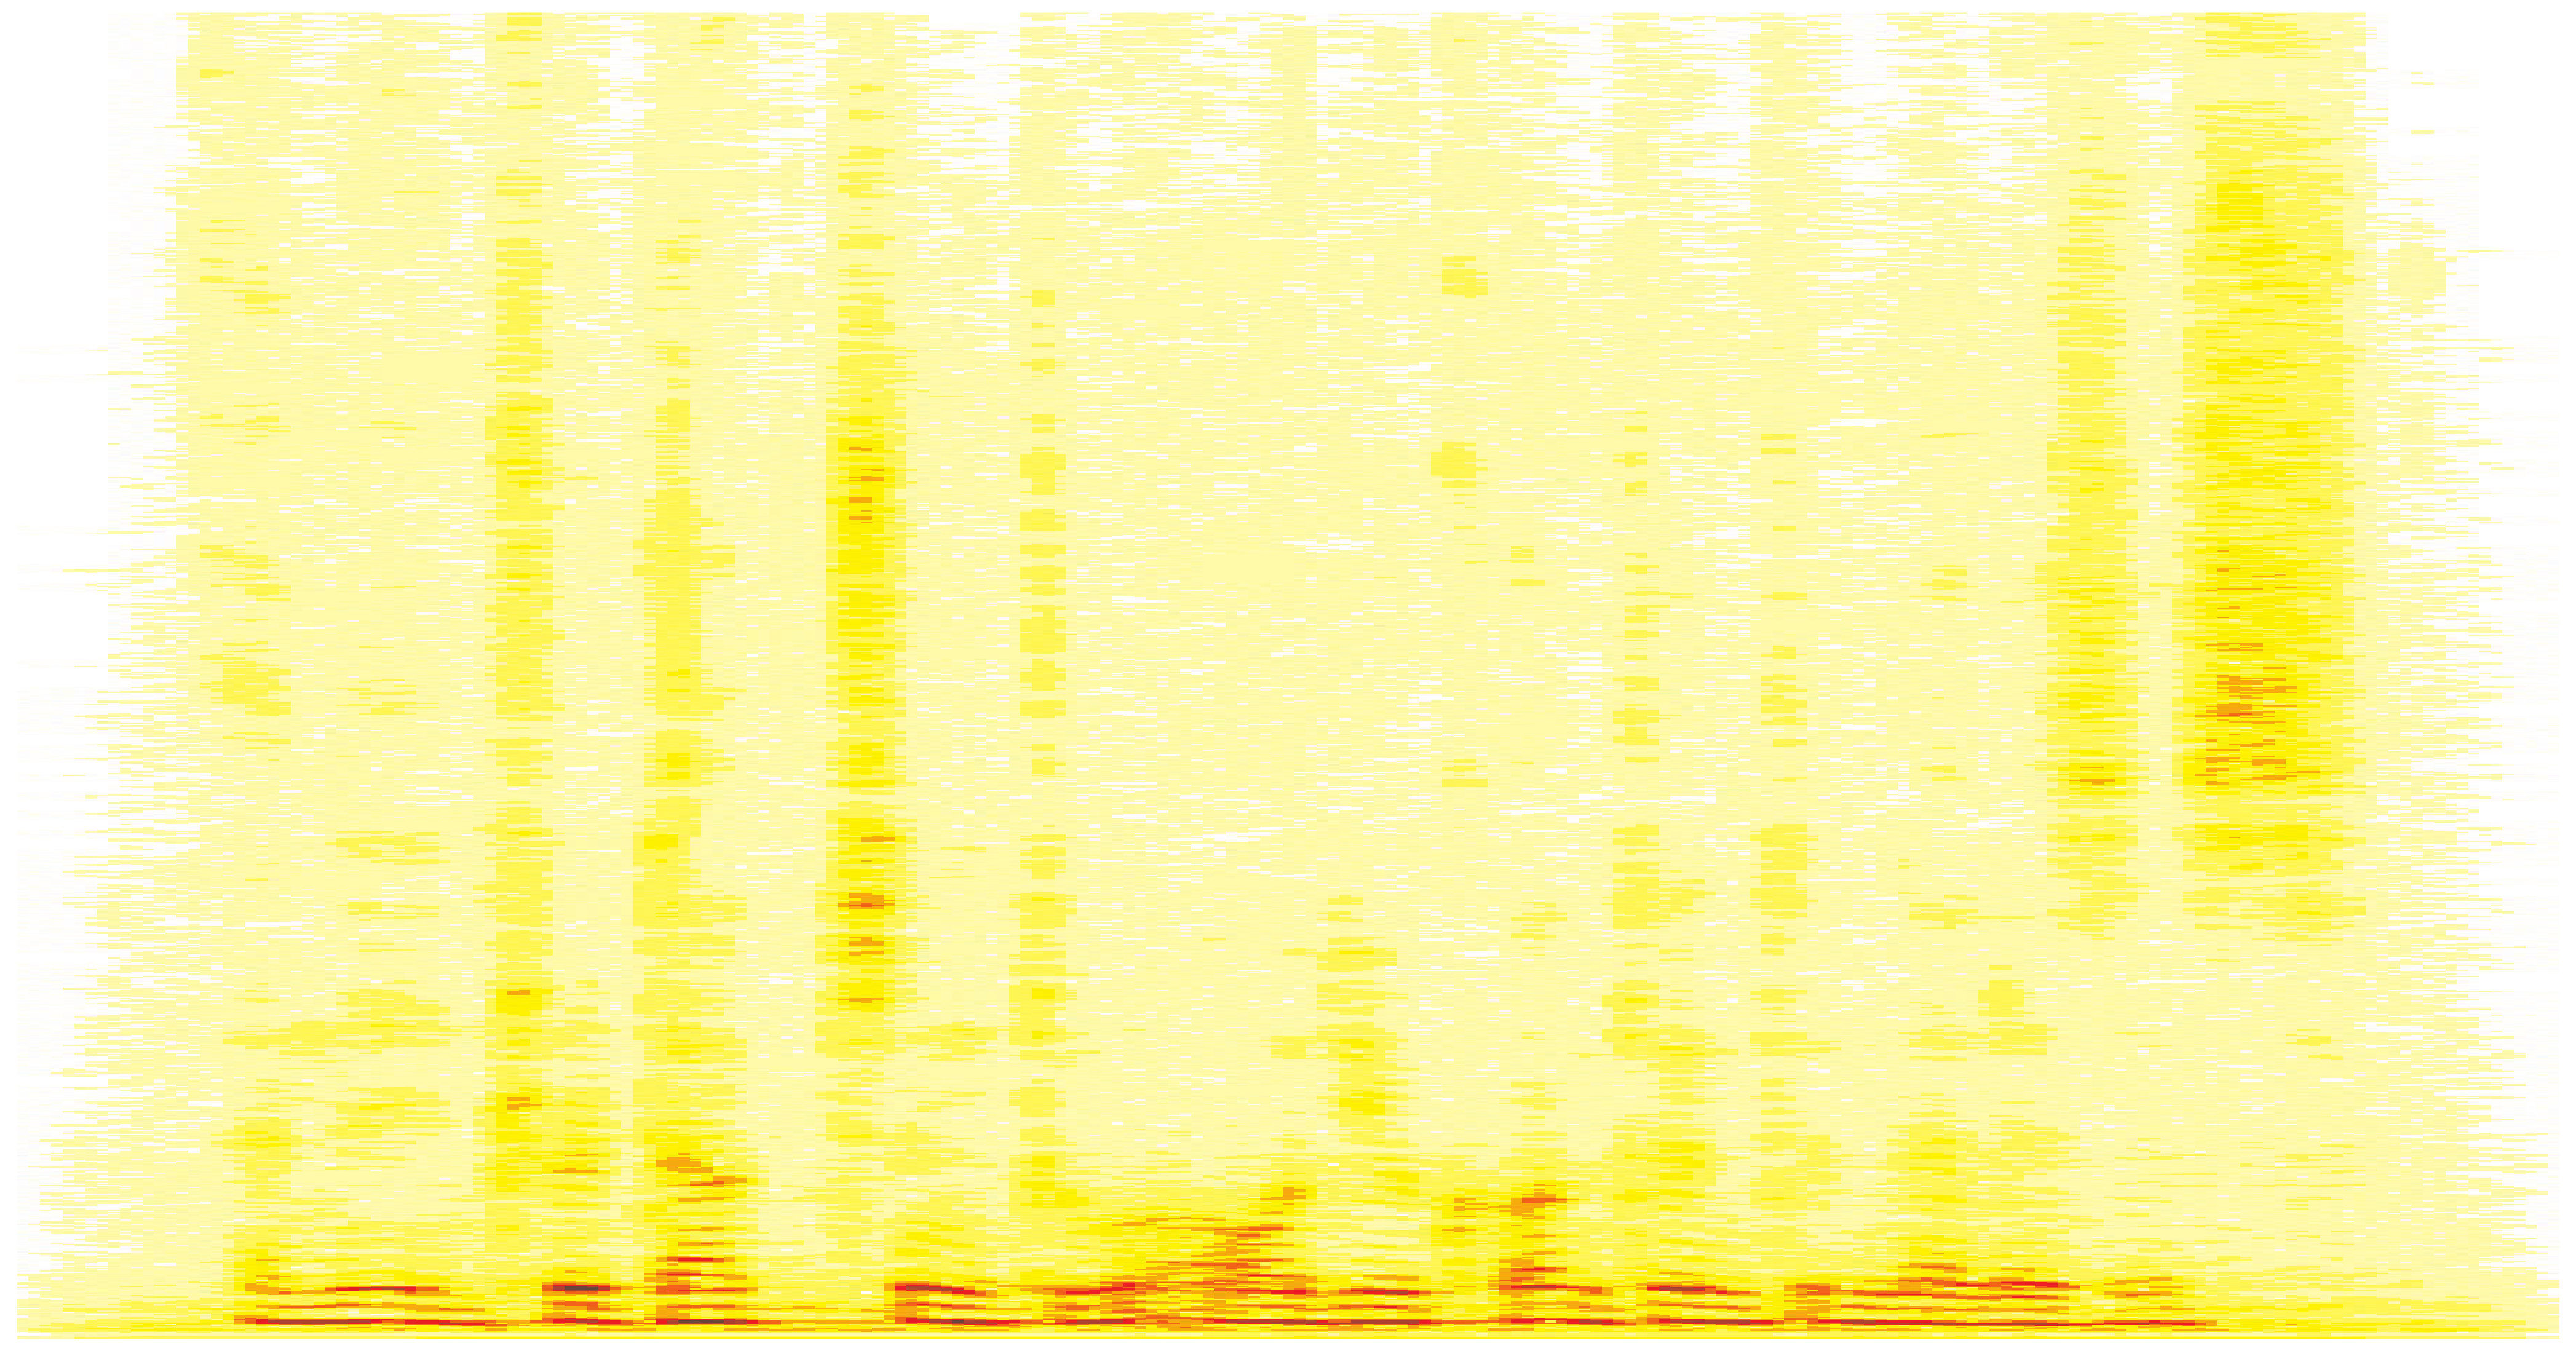
\includegraphics[width=\textwidth,height=3cm]{title}}

%%%%%%%%%%%%%%%%%%%%%%%%%%%%%%%%%%%%%%%%%%%%%%%%%%%%%%%%%%%%%%%%%%%%%%%%%%%%%%%%%%
%%%%%%%%%%%%%%%%%%%%%%%%%%%%%%%%%%%%%%%%%%%%%%%%%%%%%%%%%%%%%%%%%%%%%%%%%%%%%%%%%%
% colors
\definecolor{gtgold}{HTML}{E0AA0F} %{rgb}{0.88,0.66,1,0.06} [234, 170, 0]/256

%%%%%%%%%%%%%%%%%%%%%%%%%%%%%%%%%%%%%%%%%%%%%%%%%%%%%%%%%%%%%%%%%%%%%%%%%%%%%%%%%%
%%%%%%%%%%%%%%%%%%%%%%%%%%%%%%%%%%%%%%%%%%%%%%%%%%%%%%%%%%%%%%%%%%%%%%%%%%%%%%%%%%
% math
\DeclareMathOperator*{\argmax}{argmax}
\DeclareMathOperator*{\argmin}{argmin}
\DeclareMathOperator*{\atan}{atan}
\DeclareMathOperator*{\arcsinh}{arcsinh}
\DeclareMathOperator*{\sign}{sign}
\DeclareMathOperator*{\tcdf}{tcdf}
\DeclareMathOperator*{\si}{sinc}
\DeclareMathOperator*{\princarg}{princarg}
\DeclareMathOperator*{\arccosh}{arccosh}
\DeclareMathOperator*{\hwr}{HWR}
\DeclareMathOperator*{\flip}{flip}
\DeclareMathOperator*{\sinc}{sinc}
\DeclareMathOperator*{\floor}{floor}
\newcommand{\e}{{e}}
\newcommand{\jom}{\mathrm{j}\omega}
\newcommand{\jOm}{\mathrm{j}\Omega}
\newcommand   {\mat}[1]    		{\boldsymbol{\uppercase{#1}}}		%bold
\renewcommand {\vec}[1]    		{\boldsymbol{\lowercase{#1}}}		%bold

%%%%%%%%%%%%%%%%%%%%%%%%%%%%%%%%%%%%%%%%%%%%%%%%%%%%%%%%%%%%%%%%%%%%%%%%%%%%%%%%%%
%%%%%%%%%%%%%%%%%%%%%%%%%%%%%%%%%%%%%%%%%%%%%%%%%%%%%%%%%%%%%%%%%%%%%%%%%%%%%%%%%%
% media9
\newcommand{\includeaudio}[1]{{\includemedia[
                        addresource=audio/#1.mp3,
                        width=5mm,
                        height=5mm,
                        activate=onclick,
                        flashvars={
                            source=audio/#1.mp3  
                            &autoPlay=true
                        }]
                        {
\includegraphics[width=5mm, height=5mm]{SpeakerIcon}}
                        {APlayer.swf}}}
\newcommand{\audioautoplay}[1]{{\begin{center}\includemedia[
                            addresource=audio/#1.mp3,
                            width=.1\linewidth,
                            height=.01\linewidth,
                            activate=pageopen,
                            flashvars={
                                source=audio/#1.mp3  
                                &autoPlay=true
                            }]
                            {}
                            {APlayer.swf}\end{center}}}

\newcommand{\includevideo}[1]{{\begin{center}\includemedia[
                        addresource=video/#1.mp4,
                        width=0.8\linewidth,
                        height=0.4\linewidth,
                        activate=onclick,
                        flashvars={
                            source=video/#1.mp4  
                            &autoPlay=true
                        }]
                        {}
                        {VPlayer.swf}\end{center}}}
\newcommand{\videowithmatlab}[1]{{\begin{center}\includemedia[
                        addresource=video/animate#1.mp4,
                        width=0.8\linewidth,
                        height=0.4\linewidth,
                        activate=onclick,
                        flashvars={
                            source=video/animate#1.mp4  
                            &autoPlay=true
                        }]
                        {}
                        {VPlayer.swf}\end{center}\addreference{matlab source: matlab/animate#1.m}}}
                        

%%%%%%%%%%%%%%%%%%%%%%%%%%%%%%%%%%%%%%%%%%%%%%%%%%%%%%%%%%%%%%%%%%%%%%%%%%%%%%%%%%
%%%%%%%%%%%%%%%%%%%%%%%%%%%%%%%%%%%%%%%%%%%%%%%%%%%%%%%%%%%%%%%%%%%%%%%%%%%%%%%%%%
% other commands
\newcommand{\question}[1]{%\vspace{-4mm}
                          \setbeamercovered{invisible}
                          \begin{columns}[T]
                            \column{.8\textwidth}
                                \textbf{#1}
                            \column{.2\textwidth}
                                \vspace{-8mm}
                                \begin{flushright}
                                     
\includegraphics[scale=.5]{question_mark}
                                \end{flushright}
                                \vspace{6mm}
                          \end{columns}\pause\vspace{-12mm}}

\newcommand{\toremember}[1]{%\vspace{-4mm}
                          \begin{columns}[T]
                            \column{.8\textwidth}
                                \textbf{#1}
                            \column{.2\textwidth}
                                \vspace{-4mm}
                                \begin{flushright}
                                     
\includegraphics[scale=.5]{exclamation_mark}
                                \end{flushright}
                                \vspace{6mm}
                          \end{columns}\vspace{-6mm}}

\newcommand{\matlabexercise}[1]{%\vspace{-4mm}
                          \setbeamercovered{invisible}
                          \begin{columns}[T]
                            \column{.8\textwidth}
                                \textbf{matlab exercise}: #1
                            \column{.2\textwidth}
                                \begin{flushright}
                                     
\includegraphics[scale=.5]{logo_matlab}
                                \end{flushright}
                                %\vspace{6mm}
                          \end{columns}}

\newcommand{\addreference}[1]{  
                  
                    \begin{textblock*}{\baselineskip }(1.12\textwidth,.3\textheight) %(1.15\textwidth,.4\textheight)
                        \rotatebox{90}{\tiny {#1}}
                    \end{textblock*}}
                    
\newcommand{\figwithmatlab}[1]{
                    \begin{figure}
                        \centering
                        \includegraphics{#1}
                        %\label{fig:#1}
                    \end{figure}
                    
                    \addreference{matlab source: \href{https://github.com/alexanderlerch/ACA-Slides/blob/master/matlab/display#1.m}{matlab/display#1.m}}}
\newcommand{\figwithref}[2]{
                    \begin{figure}
                        \centering
                        \includegraphics{#1}
                        \label{fig:#1}
                    \end{figure}
                    
                    \addreference{#2}}  
                                    
\newcommand{\inserticon}[1]{

                    \begin{textblock*}{100mm}(14.5cm,7.5cm)
                        \includegraphics[height=.8cm,keepaspectratio]{#1}
                    \end{textblock*}}            

%%%%%%%%%%%%%%%%%%%%%%%%%%%%%%%%%%%%%%%%%%%%%%%%%%%%%%%%%%%%%%%%%%%%%%%%%%%%%%%%%%
%%%%%%%%%%%%%%%%%%%%%%%%%%%%%%%%%%%%%%%%%%%%%%%%%%%%%%%%%%%%%%%%%%%%%%%%%%%%%%%%%%
% counters
\newcounter{i}
\newcounter{j}
\newcounter{iXOffset}
\newcounter{iYOffset}
\newcounter{iXBlockSize}
\newcounter{iYBlockSize}
\newcounter{iYBlockSizeDiv2}
\newcounter{iDistance}



\subtitle{Module 2.6: Fundamentals~---~Non-Fourier Time-Frequency Transforms}

%%%%%%%%%%%%%%%%%%%%%%%%%%%%%%%%%%%%%%%%%%%%%%%%%%%%%%%%%%%%%%%%%%%%%%%%%%%%
\begin{document}
    % generate title page
	

\begin{frame}
    \titlepage
    %\vspace{-5mm}
    \begin{flushright}
        \href{http://www.gtcmt.gatech.edu}{\includegraphics[height=.8cm,keepaspectratio]{logo_GTCMT_black}}
    \end{flushright}
\end{frame}


    \section[overview]{lecture overview}
        \begin{frame}{introduction}{overview}
            \begin{block}{corresponding textbook section}
                    \href{http://ieeexplore.ieee.org/xpl/articleDetails.jsp?tp=&arnumber=6331119&}{Chapter 2~---~Fundamentals}: pp.~9--11
            \end{block}

            \begin{itemize}
                \item   \textbf{lecture content}
                    \begin{itemize}
                        \item   constant-Q transform (CQT)
                        \item   Gammatone filterbank
                    \end{itemize}
                \bigskip
                \item<2->   \textbf{learning objectives}
                    \begin{itemize}
                        \item   discussing the advantages and disadvantages of different time-frequency transforms
                        \item   explaining the principles of the CQT and auditory filterbanks
                    \end{itemize}
            \end{itemize}
            \inserticon{directions}
        \end{frame}
        
    \section[intro]{introduction}
        \begin{frame}{other time frequency transforms}{introduction}
            \begin{itemize}
                \item   Fourier transform continues to be much-used tool in audio signal processing and MIR
                \bigskip
                \item   but there are disadvantages, e.g.
                    \begin{itemize}
                        \item   frequency axis does not directly map to (perceptual) pitch axis
                        \item   frequency and time resolution inversely related
                        \smallskip
                        \item<2->[$\Rightarrow$] \textbf{alternative transforms} can be used
                    \end{itemize}
            \end{itemize}
        \end{frame}
        
    \section[CQT]{constant-Q transform}
        \begin{frame}{constant-Q transform}{introduction}
            \begin{itemize}
                \item<1-> DFT has a \textit{linear} frequency axis:
                    \begin{itemize}
                        \item	not perceptually meaningful: \textit{logarithmic} is better match
                        \item	low frequency resolution at low frequencies
                    \end{itemize}
                \bigskip
                \item<2->[$\Rightarrow$] compute DFT-like transform {\color{gtgold}{at specific frequencies}}
                    \begin{itemize}
                        \item   space frequencies logarithmically (constant $\mathcal{Q}$)
                        \item   resulting abscissa resolution is pitch-related
                    \end{itemize}
            \end{itemize}
            
            \bigskip
            \visible<2->{\begin{equation*}
                \mathcal{Q} = \frac{f}{\Delta f} = \frac{1}{2^{\nicefrac{1}{c}}-1}
            \end{equation*}
            }
        \end{frame}	

        \begin{frame}{constant Q transform}{implementation 1/2}
            
            \begin{columns}
            \column{0.55\textwidth}
            \begin{eqnarray*}
                X_\mathrm{CQ}(k,n) &=& \frac{1}{\mathcal{K}(k)}\sum\limits_{i=i_{\mathrm{s}}(n)}^{i_{\mathrm{e}}(n)}{w_k(i-i_{\mathrm{s}})\cdot x(i) \e^{\mathrm{j}2\pi \frac{\mathcal{Q}\cdot(i-i_{\mathrm{s}})}{\mathcal{K}(k)}}}\\
                \mathcal{K}(k) &=& \frac{f_{\mathrm{S}}}{f(k)} \mathcal{Q}
            \end{eqnarray*} 
            
            \column{0.45\textwidth}
            \begin{itemize}
                \item   $f(k)$: frequency of bin index $k$
                \item   $\mathcal{K}(k)$: blocklength for bin index $k$
                \item   $\mathcal{Q}$: measure of pitch res.
                \item   $w_k$: window function
                \item   $i_\mathrm{s},i_\mathrm{e}$: start and stop time indices of block
                \item   $f_\mathrm{S}$: sample rate
            \end{itemize}
            \end{columns}
            \bigskip
            \begin{itemize}
                \item   long window for low frequencies (high freq res, low time res)
                \item   short window for high frequencies (low freq res, high time res)
            \end{itemize}
        \end{frame}	

        \begin{frame}{constant Q transform}{implementation 2/2}
            \vspace{-5mm}
            \begin{columns}
                \column{.4\linewidth}
                    \begin{center}\textbf{non-overlapping}\end{center}
                    \vspace{-8mm}
                    \begin{figure}
                    \centering
                        \scalebox{1.2}{\newcommand{\plotrect}[1]{%
\setcounter{iXOffset}{0}%
\setcounter{i}{0}%
\whiledo{\value{i} < #1}%
{%
    \put(\value{iXOffset}, \value{iYOffset})%
        {\framebox(\value{iXBlockSize}, \value{iYBlockSize})}%
    \addtocounter{iXOffset}{\value{iXBlockSize}}%
    \stepcounter{i}%
}%                    
\addtocounter{iYOffset}{\value{iYBlockSize}}%
\addtocounter{iYBlockSize}{\value{iYBlockSize}}%
}

\begin{footnotesize}
				\begin{picture}(18,40)
					\setcounter{iYOffset}{5}
					\setcounter{iXBlockSize}{16}
					\setcounter{iYBlockSize}{1}
	
					% blocks
                    \plotrect{\value{iYBlockSize}}

					\setcounter{iXBlockSize}{8}
                    \plotrect{\value{iYBlockSize}}

					\setcounter{iXBlockSize}{4}
                    \plotrect{\value{iYBlockSize}}

					\setcounter{iXBlockSize}{2}
                    \plotrect{\value{iYBlockSize}}

					\setcounter{iXBlockSize}{1}
                    \plotrect{\value{iYBlockSize}}

					\put(9,69)
						{\text{5-point CQT}}
					\put(6,2)
						{\text{time}}
					\put(-5, 15)
						{\rotatebox{90}{\text{frequency}}}
				\end{picture}
\end{footnotesize}
}
                    \end{figure}
                \column{.6\linewidth}
                    \begin{center}\textbf{overlapping}\end{center}
                    \vspace{10mm}
                    \begin{itemize}
                        \item   define transformation matrix with maximum window length
                        \item   zeropad higher frequencies (left \& right)
                        \bigskip
                        \item[$\Rightarrow$] independent definition of block and hop length
                    \end{itemize}
                    \vspace{15mm}
                \end{columns}
        \end{frame}	

        \begin{frame}{constant Q transform}{CQT vs.\ DFT}
            \textbf{CQT}:
            \bigskip
            \begin{itemize}
                \item<1->[+]	perceptually/musically adapted frequency resolution
                \smallskip
                \item<2->[--]	time resolution depends on frequency
                \smallskip
                \item<3->[--]	not invertible
                \smallskip
                \item<4->[--]	no optimized implementation (compare FFT)
            \end{itemize}
        \end{frame}	

    \section{Auditory Filterbanks}
        \begin{frame}{auditory filterbanks}{introduction}
            FT and related transforms bad models of physiological properties of the human ear:
                \begin{itemize}
                    \item   frequency resolution (critical bands)
                    \item   frequency scale (pitch resolution)
                    \item   loudness \& masking
                    \item   event perception \&  time integration
                \end{itemize}
            
            \smallskip
            $\Rightarrow$ \textbf{auditory filterbanks}
            
            \pause
            \bigskip
            not as widely used as one might think because
            
            \begin{enumerate}
                \item<3->	computationally inefficient
                \item<3->	analysis only: no invertibility (mostly)
                \item<3->	not proven to be superior
            \end{enumerate}
        \end{frame}	

        \begin{frame}{auditory filterbanks}{gammatone filterbank}
            \vspace{-6mm}
            \begin{equation*}
                h(i) = \frac{ a \cdot\left(\nicefrac{i}{f_{\mathrm{S}}}\right)^{\mathcal{O}-1}\cdot \cos\left( 2\pi \cdot f_{\mathrm{c}} \frac{ i}{f_{\mathrm{S}}} \right) }{\e^{\nicefrac{2\pi i \Delta f}{f_{\mathrm{S}}}}}
            \end{equation*}
            \vspace{-4mm}
            \figwithmatlab{Gammatone}
        \end{frame}	

    \section{summary}
        \begin{frame}{summary}{lecture content}
            \begin{itemize}
                \item   \textbf{DFT has disadvantages}
                    \begin{itemize}
                        \item   low frequency resolution for low pitches
                        \item   non-logarithmic/perceptually relevant pitch resolution
                    \end{itemize}
                \bigskip
                \item      \textbf{CQT}
                    \begin{itemize}
                        \item   similar to Fourier Transform but logarithmically spaced frequency bins
                        \item   not invertible and inefficient
                    \end{itemize}
                \bigskip
                \item      \textbf{Filterbanks}
                    \begin{itemize}
                        \item   good model of human physiology
                        \item   not invertible and inefficient
                        \item   not proven to be superior
                    \end{itemize}
            \end{itemize}
            \inserticon{summary}
        \end{frame}
\end{document}
